\documentclass{article}
\usepackage[utf8]{inputenc}
\usepackage{setspace}

%% Sets page size and margins
\usepackage[a4paper,top=3cm,bottom=2cm,left=3cm,right=3cm,marginparwidth=1.75cm]{geometry}

%% Useful packages
\usepackage{listings}
\usepackage{caption}
\usepackage{amssymb,amsmath,amsthm}
\usepackage{mathtools} \usepackage{graphicx}
\usepackage[colorlinks=true, allcolors=blue]{hyperref}
\usepackage{float}
\usepackage[table,xcdraw]{xcolor}
\usepackage{enumerate}
\usepackage{subcaption}
\usepackage{hyperref}
\newcommand{\Lagr}{\mathcal{L}}
\newcommand\norm[1]{\left\lVert#1\right\rVert}
\DeclareMathOperator*{\argmin}{arg\,min} 
\usepackage{tikz-cd}
\usepackage{amsthm}
\newtheorem{theorem}{Theorem}
\theoremstyle{definition}
\newtheorem{definition}{Definition}

\newtheorem*{proposition}{Proposition}
\newtheorem*{corollary}{Corollary}
\newtheorem*{example}{Example}
\newtheorem*{lemma}{Lemma}
\newtheorem{observation}{Observation}

\usepackage{fancyhdr}
\pagestyle{fancy}
\thispagestyle{empty}
\onehalfspacing

\begin{document}

\title{SuperResolution}

\author{José Pablo Ortiz}
\maketitle

\section{Introduction}
In this work there is concise presentation of convolutional neural networks(CNN) and an architecture, the UNet, that uses CNN. The purpose
\section{Signals}
A \textbf{bidimentional discrete signal} is an infinite matrix with entries $x_{ij}$, where $x_{ij}$ is the activation of the position $(i,j)$[Calin]. The entries $x_{ij}$  have a spatial relationship according to their position $(i,j)$. An example of bidimentional discrete signal is a grey scale digital image where $x_{ij}=1$ means that the pixel $(i,j)$ is black; while $x_{ij}=0$ means that the pixel $(i,j)$ is white, and any number between 0 and 1 is a grey tone.

\noindent
A bidimentional discrete signal is called finite support if there exsists $K$ such that for every $|i|>K$ and $|j|>K$ $x_{ij}= 0$; then, this kind of signal can be represented as a finite matrix. In this work, we will only focus on finite supports signals. in order to explain the theory behind convolutional neural networks we need to make some definitions. 



\begin{definition}
Let $X$ be a matrix and  $S,P\subseteq \mathbb{N}$ sets of contiguous natural numbers. The submatrix with rows $S$ and columns $p$ will be denoted by $X_{S,P}$ and will be called contiguous submatrix.
\end{definition}
\noindent
We are trying to create an expansion of $X$ which contains some or all of the contiguous submatrices of $X$ of dimension $m_1$ and $m_2$. For this end we define the following sets
\begin{equation}
S_i=\{1+is-1,\dots,m_1+is-1\}\quad P_j = \{1+pj-1,\dots,m_2+pj-1\}.
\end{equation}
The numbers $s,p\in\mathbb{N}$  are called height and width stride. They represen the separation that exsists between the contiguous submatrices. On the other hand, in order for the contiguous submatrix to be well defined the values of $i$ and $j$ need to be:
$$i= 1,\dots,\frac{n_1-m_1+1}{s}\quad j= 1,\dots,\frac{n_2-m_2+1}{p}. $$

\begin{definition}
The contiguous submatrix expansion of dimension $m_1$ and $m_2$ with strides $s$ and $p$ of the matrix $X$ is given by the following block matrix
\begin{equation}
\mbox{c.s.e.}(X;m_1,m_2,s,p) = \begin{pmatrix}
A_{S_1,J_1}&\dots& A_{S_1,J_{k_2}}\\
\vdots & \ddots & \\
A_{S_{k_1},P_1}&\dots&A_{S_{k_1},P_{k_2}}
\end{pmatrix},
\end{equation}
where  $S_i$ and $P_j$ are defined as in (1) with $k_1= \frac{n_1-m_1+1}{s}$ and $k_2=\frac{n_2-m_2+1}{p}$.
\end{definition}
\noindent
This expansion can be seen as block matrix with all the rolling windows of dimension $m_1$ and $m_2$ with stride $s$ and $p$. Once we have the expansion in (2) is quite easy to give an outline of how convolution neural networks work.

\section{Convolutional operator}
\begin{definition}
The convolutional operator  $\circledast$ between a signal $X$ and   $W\in\mathbb{R}^{(m_1\times m_2)}$  with stride $(s,p)$ is the matrix $Z =X\circledast W $ where the entries are given by 
\begin{equation*}
\begin{split}
z_{ij} &=\sum_{u=s_i}^{s_i+m_1}\sum_{v=p_j}^{p_j+m_2}a_{uv}w_{uv}\\
&=1_{m_1}^T(X_{S_i P_j}\odot W)1_{m_2}
\end{split}
\end{equation*}
where $X^{(k)}_{S_i,P_j}$ is the contiguous submatrix of $\mbox{c.s.e.}(X;m_1,m_2,s,p) $ and $s_i=\min(S_i)$ an $p_j=\min(P_j)$. 
\end{definition}
\noindent
Let $X$ be an image in grey scale, within the context of convolutional neural netwroks, $W$ is called filter or kernel because after convolving $X$ and $W$; $W$ has the capacity to obtain features from $X$. Thus, the resulting matrix $Z=X\circledast W$ it is called \textbf{feature map}. Figure 1 in an example of this; where a kernel $W$ was applied to $X$ to obtain the outlines of the image. 
\begin{figure}[H]
\centering
\begin{subfigure}{.5\textwidth}
  \centering
  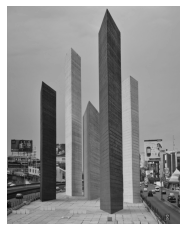
\includegraphics[width=.5\linewidth]{Imagenes/satelite.png}
  \caption{A subfigure}
  \label{fig:sub1}
\end{subfigure}%
\begin{subfigure}{.5\textwidth}
  \centering
  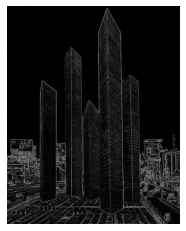
\includegraphics[width=.5\linewidth]{Imagenes/satelite_outline.png}
  \caption{A subfigure}
  \label{fig:sub2}
\end{subfigure}
\caption{A figure with two subfigures}
\label{fig:test}
\end{figure}

\subsection{Multiple channel convolution}
In a more broad context and image $X\in\mathbb{R}^{(n_1\times n_2)\times c}$ is a tensor where $c$ is the number of channels in the image. The number of channels represents the number of characteristics that we have a bout $X$; and the entry $x_{ijk}$ tha value of the $k$-th characteristic at the position $(i,j)$. For example, in a RGB image  $X\in\mathbb{R}^{(n_1\times n_2)\times 3}$ and every entry $x_{ij}=[r_{ij1},g_{ij2},b_{ij3}],$is a combination of the different intensity of the primary colors(red, green and blue). To ease the notation the matrix $X[:,:,k]$ will denote the feature map of the $k$ characteristic or channel.

\noindent
El número de canales representa la cantidad de características que se tienen de $X$; y la entrada $x_{ijk}$
el valor la $k$-ésima característica en la posición $(i,j)$. Por ejemplo, una imagen del tipo RGB $X\in\mathbb{R}^{(n_1\times n_2)\times 3}$ y cada entrada $x_{ij}=[r_{ij1},g_{ij2},b_{ij3}],$ es una combinación de diferentes intensidades de los colores primarios; \textit{red, green, blue} por sus nombres en ingles.

\begin{definition}
The convolutional operator $\circledast$  between $X\in\mathbb{R}^{(n_1\times n_2)\times c}$ a multiple channel signal and $W\in\mathbb{R}^{(m_1\times m_2)\times c}$ with stride $(s,p)$ is the matrix $Z=X\circledast W$ with entries 
\begin{equation*}
\begin{split}
z_{ij} &=\sum_{k=1}^{c}\sum_{u=s_i}^{s_i+m_1}\sum_{v=p_j}^{p_j+m_2}x_{uvk}w_{uvk}\\
&=\sum_{k=1}^{c} 1_{m_1}^T(X[:,:,k]_{S_i P_j}\odot W^{(k)})1_{m_2}
\end{split}
\end{equation*}
where $X[:,:,k]_{S_i P_j}$ is the contiguos submatrix of  $e.s.c.(X[:,:,k];m_1,m_2,s,p)$, $s_i=\min(S_i)$ and $p_j=\min(P_j)$. 
\end{definition}
\noindent
In words, it's the sum of the convolution between each channel of $X$ and $W$. This type of convolution is useful because the filter $W$ moves around the spatial positions of $X$.

\section{Resampling}
Resampling is the process of changing the sampling rate or sampling frequency of a discrete signal to obtain a new discrete representation of the underlying continuous signal.[Oppenheim, Alan V.; Schafer, Ronald W.; Buck, John R. (1999). Discrete-time signal processing]. In this project we will two types of resampling methods: DownSampling and UpSampling. When working with images DownSampling is the process of reducing the size of the image and UpSampling is the process of increasing the size of the image. There are many DownSampling and UpSampling techniques; nonetheless, in this project for DownSampling we will use max pooling and for UpSampling nearest-neighbor interpolation.

\begin{definition}
Let $X\in\mathbb{R}^{n_1\times n_2}$  maxPooling operator of dimension $m_1$ and $m_2$ and stride $(s,p)$
\begin{equation}
z_{ij}=\max(A_{S_iP_j}),
\end{equation}
where $A_{S_iP_j}$ is the block matrix of $\mbox{c.s.e.}(X;m_1,m_2,s,p)$.
\end{definition}
Then if $Z = \mbox{maxPool}(A;m_1,m_2,s,p)$  is a matrix of size $k_1$ and $k_2$. When $X$ is a multiple channel signal then the maxPooling operator is applied individually to every channel.


\section{Layers}
The layers that almost all CNN architectures use are convolutional, maxPooling and dropout. Nonetheless, in this application we will also use an UpSampling image.

\subsection{Convolution Layer}
 The input of this layers is a feature map $X\in\mathbb{R}^{(n_1\times n_2)\times c_0}$ and the output is another feature map $Z\in\mathbb{R}^{(n_1\times n_2)\times c_1}$. In this layer we apply multiple channel convolutions between  $X$ and $c_1$ kernels of size $(m_1,m_2)$ with both the  stride width and height equal to 1. Each of this kernels consists of the weights/parameters that need to be estimated. Let $W\in\mathbb{R}^{[(n_1\times n_2)\times c_0]\times c_1}$ be the $c_1$ kernels that need to be estimated then we define $\hat{Z}\in\mathbb{R}^{(n_1\times n_2) \times c_1}$ as 

\begin{equation}
\hat{Z}[:,:,k]=X\circledast W[:,:,:,k].
\end{equation}
The convolutional layer ends with the applicacion of the ReLU activation function, that is:
\begin{equation}
z_{ijk}= \max{(0,\hat{z}_{ijk})}.
\end{equation}
The reason a ReLU activation function is used is to add non linearity and to make the model more sparse by removing weak characteristics. This layer is the only one that has weights/parameters that need to be estimated.

\subsection{MaxPooling Layer}
The maxPooling layer has as input a feature map $X\in\mathbb{R}^{(n_1\times n_2)\times c_0}$ and consists of applying maxPooling to each of the characteristics of $X$. That is, if $Z=\mbox{maxPooling}(X;m_1,m_2,s,p)$ then 
\begin{equation}
	z_{ijk} = \max(X[:,:,k]_{S_iP_j})
\end{equation}
and $Z\in\mathbb{R}^{(k_1\times k_2)\times c_0}$.
\subsection{UpSampling Layer}
The UpSampling Layer  has as input a feature map $X\in\mathbb{R}^{(n_1\times n_2)\times c_0}$ and consists of applying the nearest-neighbor interpolation upSampling algorithm to upscale by 100$\%$ . Thus, the output will be $Z\in\mathbb{R}^{(2n_1 \times 2n_2)\times c_0}$

\section{UNet}
In this section we will present a method to UpSample an image from size $16\times 16$ to size $32\times 32$. For this end, we will use the UNet.The UNet was introduced by in 2015. And it can be classified as convolutional Encoder-Decoder. 'Encoder-Decoder models are a family of models which learn to map data-points from an input domain to an output domain via a two-stage network: The encoder, represented by an encoding function $z = f(x)$, compresses the input into a latent-space representation; the decoder, $y = g(z)$, aims to predict the output from the latent space representation.'[cita]

\noindent
Both the Encoder and the Decoder are convolutional neural networks in blocks. A block is a combination of successive applications of the layers in section 5. The innovation of the UNet is that each block of the Decoder is connected to a block in the Encoder. The blocks used in the encoder will be called Down Block and the blocks used in the decoder will be called Up Block.

\subsection{Down Block}
Figure 2 shows the composition of a DownBlock.  'It consists of the repeated application of two 3x3 convolutions (same convolutions), each followed by a rectified linear unit (ReLU) and a 2x2 max pooling operation with stride 2 for downsampling. At each downsampling step we double the number of feature channels.'[cita]

\subsection{Up Block}
Figure 2 shows the composition of a UpBlock. 'Every step in the expansive path consists of an upsampling of the feature map followed by a 2x2 convolution that halves the number of feature channels, a concatenation with the correspondingly cropped
feature map from the contracting path, and two 3x3 convolutions, each followed by a ReLU'.[cita]

\begin{figure}[h]
    \centering
    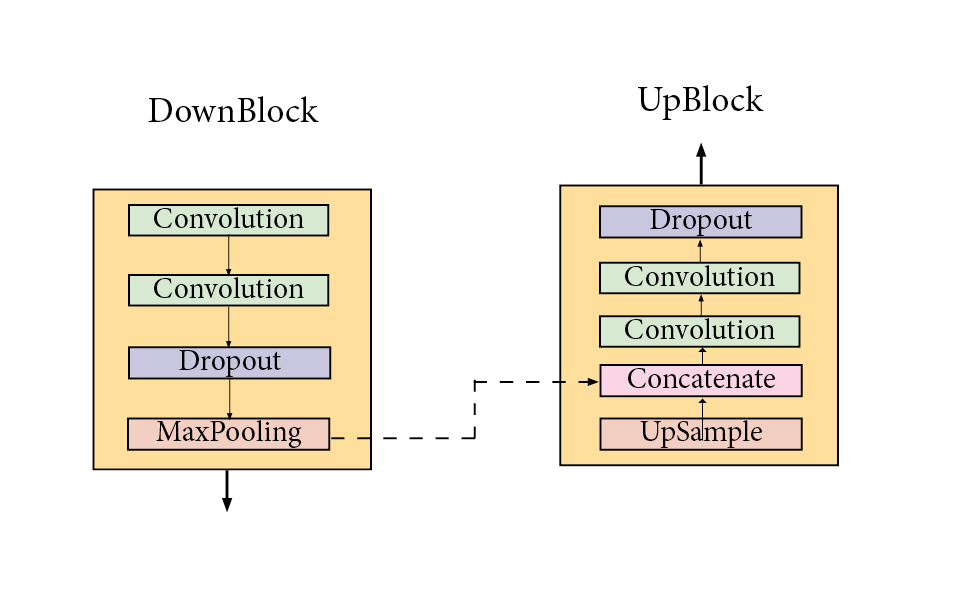
\includegraphics[width=0.7\textwidth]{Imagenes/DownUp.png}
    \caption{The DownBlock and UpBlock along with the connection they have.}
    \label{fig:mesh1}
\end{figure}

\subsection{Tail}
The tail consists of an UpSample layer followed by two 3x3 convolutions, each followed by a ReLU.

\subsection{Model}
 Figure 3 shows the architecure of the Unet used in order to up sample an image by 2x. Hence, the model is a function $f_\theta:\mathbb{R}^{(16\times 16)\times 3}\rightarrow \mathbb{R}^{(32\times 32)\times 3}$ where $\theta$ is all the matrices $W$ given in a convolutional layer. 
\begin{figure}[h]
    \centering
    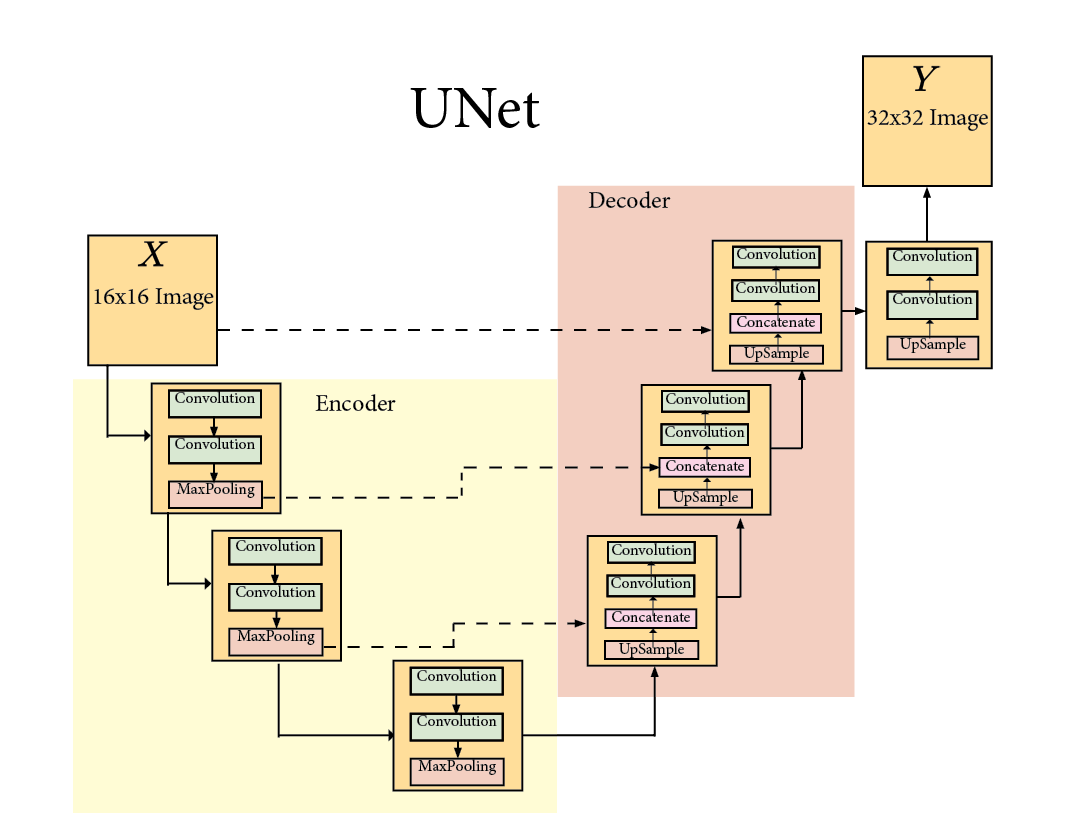
\includegraphics[width=0.7\textwidth]{Imagenes/Unet2.png}
    \caption{TheUNet: in yellow the encoder and in red the decoder.}
    \label{fig:mesh1}
\end{figure}

\section{Training}

\subsection{Dataset and preproces}
The dataset was gather from Wikipedia and it consisted in images of famous paintings from different periods and places. Then we gather all the contiguous submatrix of size $(32,32)$ with stride $(32,32)$. Everyone of this images of size $(32,32)$  was then downsample using nearest-neighbor interpolation to a size of $(16,16)$. 

\noindent
The dataset will be have as inputs the images of size $(16,16)$, $X\in\mathbb{R}^{(16\times 16)\times 3}$, and outpus the corresponding images of size $(32,32,3)$, $Y\in\mathbb{R}^{(32\times 32)\times 3}$. Thus, our data will have $n=23300$ observations which was split with $90\%$ training and $10\%$ test.



\subsection{Loss}
Thus, given an observation $(X,Y)$ the loss for a observation will be given by the Frobenius norm  of the difference:
\begin{equation}
L(X,Y) = \sum_{(X,Y)\in\mbox{train}}\|f_\theta(X)-Y\|_{F}.
\end{equation}  
The algorithm that it's used to minimize (7) is minibatch stochastic gradient descent with the gradient calculated through backpropagation and being updated using the ADAM method. 

\section{Results}
The results will be compared to an example given in wikipedia[Image scaling Deep convolutional neural networks], where an image of painting by Evelyn De Morgan is upscaled using different software/techniques: PaintShop Pro,  waifu2x and Topaz A.I. Gigapixel with Low noise reduction.
\pagebreak

\begin{figure}[h]
\centering
\begin{minipage}{.5\textwidth}
  \centering
  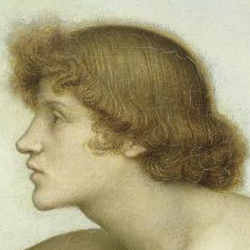
\includegraphics[width=.8\linewidth]{Imagenes/Phosphorus_and_Hesperus_original.png}
  \captionof{figure}{Original}
  \label{fig:test1}
\end{minipage}%
\begin{minipage}{.5\textwidth}
  \centering
  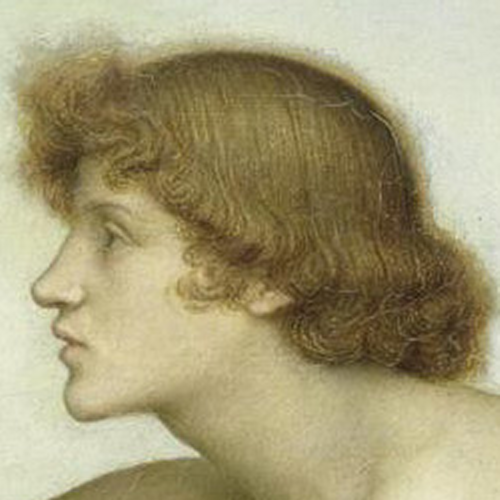
\includegraphics[width=.8\linewidth]{Imagenes/Phosphorus_and_Hesperus_Paint_Shop_Pro.png}
  \captionof{figure}{PaintShop Pro}
  \label{fig:test2}
\end{minipage}
\end{figure}


\begin{figure}[h]
\centering
\begin{minipage}{.5\textwidth}
  \centering
  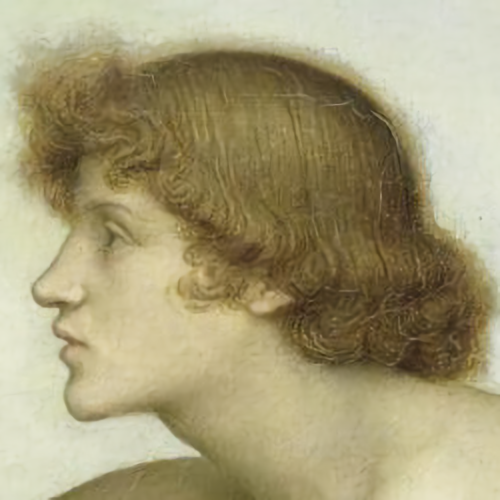
\includegraphics[width=.8\linewidth]{Imagenes/Phosphorus_and_Hesperus_Waifu2x.png}
  \captionof{figure}{Waifu2x}
  \label{fig:test1}
\end{minipage}%
\begin{minipage}{.5\textwidth}
  \centering
  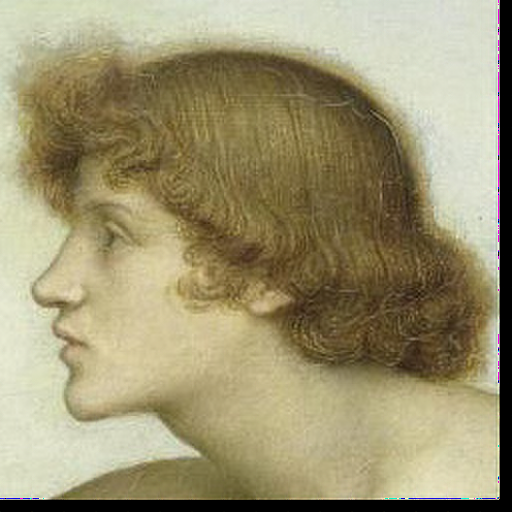
\includegraphics[width=.8\linewidth]{Imagenes/Phosphorus_and_Hesperus_UNet.png}
  \captionof{figure}{UNet}
  \label{fig:test2}
\end{minipage}
\end{figure}






\end{document}






